\documentclass[11pt]{amsart}
\usepackage{amsmath,amssymb,amsthm}
\usepackage[margin=1.1in]{geometry}
\usepackage{graphicx}
\usepackage{microtype}
\usepackage{enumitem}
\usepackage[colorlinks=true,linkcolor=blue,citecolor=blue,urlcolor=blue]{hyperref}
\setlength{\textfloatsep}{10pt plus 2pt minus 2pt}
\setlength{\floatsep}{8pt plus 2pt minus 2pt}
\setlength{\intextsep}{8pt plus 2pt minus 2pt}

\newtheorem{theorem}{Theorem}[section]
\newtheorem{lemma}[theorem]{Lemma}
\newtheorem{proposition}[theorem]{Proposition}
\newtheorem{corollary}[theorem]{Corollary}
\theoremstyle{remark}
\newtheorem{remark}[theorem]{Remark}
\newtheorem{conjecture}[theorem]{Conjecture}

\newcommand{\Z}{\mathbb{Z}}
\newcommand{\Q}{\mathbb{Q}}
\newcommand{\R}{\mathbb{R}}
\newcommand{\C}{\mathbb{C}}
\newcommand{\F}{\mathbb{F}}
\newcommand{\HH}{\mathbb{H}}
\newcommand{\cA}{\mathcal{A}}
\newcommand{\cB}{\mathcal{B}}
\newcommand{\cP}{\mathcal{P}}
\newcommand{\Sg}{\mathfrak{S}}
\newcommand{\Om}{\Omega}
\newcommand{\e}{\varepsilon}
\newcommand{\dd}{\mathrm{d}}
\newcommand{\gen}{\mathrm{gen}}
\DeclareMathOperator{\rk}{r}

\title[Sums of two squares with few prime factors]{Sums of two squares with few prime factors via theta series of quaternary forms}
\author{Ruqing Chen}
\address{GUT Geoservice Inc., Montreal, Canada}
\email{ruqing@hotmail.com}
\date{\today}

\begin{document}

\begin{abstract}
Let $N\equiv 2\pmod 4$ be large. We prove that the number of $n<N$ such that $n$ and $N-n$ are both sums of two squares, $\Omega(n(N-n))\le 9$ and $\max(\Omega(n),\Omega(N-n))\le 6$ is $\gg N/(\log N)^2$; the two bounds hold simultaneously for the same $n$. The previous bounds, obtained by sifting the primes $\equiv 3\pmod 4$ and switching, were $11$ and $8$. The new input is a level of distribution $2/5$ for the weighted sequence $r(n)r(N-n)$, where $r$ counts representations as a sum of two squares. For coprime $m,m'$ the sum $\sum_{ma+m'b=N}r(a)r(b)$ is the $N$-th coefficient of the weight-two theta series of $m(x^2+y^2)+m'(z^2+w^2)$; combining Waibel's uniform bound for the Petersson norm of the cuspidal part of a theta series with Deligne's bound through the Hecke operators, and reducing the non-coprime cases by the operators $U_p$, we obtain $\sum_{ma+m'b=N}r(a)r(b)=\text{(Siegel main term)}+O(d(N)N^{1/2}(mm')^{1/4+\e})$ uniformly in $m,m'$. In numerical experiments over a finite range the error does not grow with $mm'$; we formulate the resulting uniform bound as a conjecture, which would give the level of distribution $1/2$ and the bounds $8$ and $5$.
\end{abstract}

\maketitle

%=====================================================================================================
\section{Introduction}\label{sec:intro}

Let $r(n)=\#\{(x,y)\in\Z^2:\ x^2+y^2=n\}$, so that $r(n)=4\sum_{d\mid n}\chi(d)$ with $\chi=\chi_{-4}$ the non-trivial character modulo $4$. Every integer $N$ is a sum $n+(N-n)$ of two sums of two squares, and in \cite{Chen2} we asked for such representations in which $n$ and $N-n$ have few prime factors. For $N\equiv2\pmod4$ it was shown there, by a vector sieve in which the primes $q\equiv3\pmod4$ are sifted up to nearly $N^{1/2}$ and the survivors with two large such primes are removed by a switching argument, that there are $\gg N/(\log N)^2$ integers $n<N$ with $n$, $N-n$ sums of two squares and $\Omega(n(N-n))\le 11$, and $\gg N/(\log N)^2$ with $\max(\Omega(n),\Omega(N-n))\le 8$.

Here we take a different route: instead of sifting the primes $\equiv3\pmod 4$ we count with the weight $r(n)r(N-n)$, which vanishes unless both $n$ and $N-n$ are sums of two squares. The price is that the sequence $r(n)r(N-n)$ must be shown to be well distributed in arithmetic progressions, and the gain is that no inert prime has to be sifted and no switching is needed. We prove a level of distribution $2/5$ (Theorem~\ref{thm:level}), and the sieve then gives the following.

\begin{theorem}\label{thm:main}
Let $N\equiv2\pmod 4$ be sufficiently large. Then
\begin{multline*}
\#\bigl\{1\le n<N:\ n=x^2+y^2,\ N-n=z^2+w^2,\ \Omega(n(N-n))\le 9,\ \max(\Omega(n),\Omega(N-n))\le 6\bigr\}\\
\ge\ c_1\,\Sg_r(N)\,\frac{N}{(\log N)^2},
\end{multline*}
where $c_1>0$ is an absolute constant and
\begin{equation}\label{eq:Sr}
\Sg_r(N)=\prod_{\substack{p\mid N\\ p>2}}\rho_p,\qquad
\rho_p=\begin{cases}
\dfrac{p(p+1)(p-1)^2}{(p^2-p+1)^2} & p\equiv1\pmod 4,\\[2ex]
\dfrac{p+1}{p}\Bigl(1-\dfrac1{p(p-1)}\Bigr)^{-2} & p\equiv3\pmod 4.
\end{cases}
\end{equation}
One has $\rho_p>1$ for every $p$, so $\Sg_r(N)\ge1$. The integers counted are coprime to $N$, and each of $n$, $N-n$ is a product of distinct primes $\equiv1\pmod 4$ exceeding $N^{9/250}$.
\end{theorem}

The constant can be made explicit, $c_1=0.25$ being admissible (Section~\ref{sec:sieve}); we have not tried to optimise it. Both bounds $9$ and $6$ come from one set of sieve parameters, so they hold simultaneously for the same integers $n$. Theorem~\ref{thm:main} and the level $2/5$ are unconditional. The level $1/2$ and the bounds $8$ and $5$ discussed below are conditional on Conjecture~\ref{conj}, and are never used in the proof of Theorem~\ref{thm:main}.

\subsection*{Summary of contributions}
We separate what is proved here from what is taken from the literature.
\begin{enumerate}[label=(\alph*),leftmargin=2em]
\item \emph{The arithmetic result.} Theorem~\ref{thm:main} improves the bounds $11$ and $8$ of \cite{Chen2} to $9$ and $6$, with the same order of magnitude $N/(\log N)^2$ for the count, and with both bounds holding for the same integers.
\item \emph{A uniform coefficient bound.} The analytic input taken from the literature is Waibel's bound for the Petersson norm of the cuspidal part $G_{m,m'}$ of the theta series of a quaternary form \cite{Waibel}, together with Deligne's theorem \cite{Deligne}. A norm bound does not by itself control a single Fourier coefficient uniformly in the level: the Petersson formula applied at $n=N$ loses a factor $N^{1/4}$ when the level is small compared with $N^{1/2}$. Our contribution here is the passage from the norm to the $N$-th coefficient uniformly in $m,m'$: the part of $N$ coprime to the level is moved into a Hecke operator, whose operator norm is controlled by Deligne's bound (Lemma~\ref{lem:hecke}), and the primes of $mm'$ dividing $N$ are removed by an exact recursion with the operators $U_p$ whose coefficients we count (Lemma~\ref{lem:reduce}). The result is the uniform estimate \eqref{eq:unif} below.
\item \emph{The sieve set-up.} We prove the level of distribution $2/5$ for the weighted sequence $r(n)r(N-n)$ (Theorem~\ref{thm:level}). With this weight the inert primes have density $\ll q^{-2}$ and need not be sifted, so the sieve is a two-dimensional vector sieve of two linear components, without the switching step of \cite{Chen2}, and the final numerical inequality is correspondingly simpler (Section~\ref{sec:sieve}, Appendix~\ref{app:numerics}).
\end{enumerate}

\subsection*{The method}
Write a square-free $d$ as a product of primes $p\equiv1\pmod4$ (split) and $q\equiv 3\pmod 4$ (inert). The identities $r(n)=2r(n/p)-r(n/p^2)$ for split $p\mid n$ and $r(n)=r(n/q^2)$ for inert $q\mid n$ express the sum of $r(n)r(N-n)$ over $n\equiv0\ (d)$, $n\equiv N\ (e)$ as a combination of the sums
\begin{equation}\label{eq:T}
T(m,m';N)=\sum_{ma+m'b=N}r(a)r(b)=\#\{(x,y,z,w)\in\Z^4:\ m(x^2+y^2)+m'(z^2+w^2)=N\}
\end{equation}
with $m\mid d^2$, $m'\mid e^2$. This is the number of representations of $N$ by the positive quaternary form $Q_{m,m'}=m(x^2+y^2)+m'(z^2+w^2)$, i.e.\ the $N$-th Fourier coefficient of the theta series $\theta^2(mz)\theta^2(m'z)$, a holomorphic modular form of weight $2$ on $\Gamma_0(4mm')$. By Siegel's theorem it is the sum of the $N$-th coefficient of an Eisenstein series, which is the product $M(m,m';N)$ of the local densities, and of the $N$-th coefficient of a cusp form $G_{m,m'}$. Deligne's bound controls the latter for each fixed form, and the whole difficulty is the uniformity in the level $4mm'$. Waibel's theorem \cite{Waibel} gives $\|G_{m,m'}\|\ll(mm')^{1/4+\e}$ for our forms. Passing from the norm to the $N$-th coefficient through the Hecke operator $T_N$ rather than through the Petersson formula directly avoids a loss for small levels, and we obtain
\begin{equation}\label{eq:unif}
T(m,m';N)=M(m,m';N)+O_\e\bigl(d(N)^{4}N^{1/2}(mm')^{1/4+\e}\bigr)
\end{equation}
uniformly in coprime odd cube-free $m,m'$ (Theorem~\ref{thm:unif} and Corollary~\ref{cor:unif}; for $(N,mm')=1$ the factor $d(N)^4$ can be replaced by $d(N)$). Since the main term is of size $N/(mm')$, the error is smaller than the main term as long as $mm'\le N^{2/5-\e}$, and a bookkeeping argument turns \eqref{eq:unif} into the level of distribution $2/5$ for $r(n)r(N-n)$ (Theorem~\ref{thm:level}).

The weighted sequence has the pleasant feature that under the weight $r(n)r(N-n)$ a split prime $p$ divides $n$ with density $h(p)=(2p-1)/(p(p+1))\approx 2/p$ and an inert prime only with density $1/(q(q-1))$; so sifting all primes below $N^{\alpha}$ on both sides is a vector sieve of two linear components, and Richert's weights bound $\Omega(n(N-n))$. The numerical inequality behind Theorem~\ref{thm:main} is verified with interval arithmetic (Section~\ref{sec:sieve} and Appendix~\ref{app:numerics}).

\subsection*{Relation to the shifted convolution literature}
The sum \eqref{eq:T} is a shifted convolution problem for the coefficients of $\theta^2$ with linear coefficients $m,m'$, in the ``sum'' orientation $ma+m'b=N$. For the divisor function in place of $r$ and the ``difference'' orientation $r_1n-r_2m=h$, Topacogullari \cite{Top} proved an asymptotic formula uniform in the coefficients, with an error term of the shape $(r_2x_1)^{1/2+\vartheta+\e}$ (in his notation), where $\vartheta$ is any admissible exponent towards the Ramanujan--Petersson conjecture for Maass forms, $\vartheta=7/64$ by Kim and Sarnak \cite{KimSarnak}. The two problems are structurally different, and we do not regard one result as an improvement of the other. In the difference orientation the natural spectral expansion is over the full $L^2$ spectrum of $\Gamma_0$ of the relevant level, including Maass cusp forms, whose possible exceptional eigenvalues and non-tempered local components enter through $\vartheta$. In the sum orientation, $T(m,m';N)$ is a Fourier coefficient of a \emph{holomorphic} modular form of weight $2$, so only holomorphic cusp forms occur, Deligne's theorem gives the Ramanujan--Petersson bound at all finite places, and the uniformity in the level must instead come from a bound for the Petersson norm, which Waibel supplies. The exponent $1/4$ in \eqref{eq:unif} is the price of a Cauchy--Schwarz step in the passage from the norm of $G_{m,m'}$ to a single coefficient. Numerically (Section~\ref{sec:numerics}) the quantity $\sup_N|T-M|/\sqrt N$ does not grow with $mm'$, while the root mean square decreases like $(mm')^{-1/4}$; this is consistent with Waibel's bound being sharp up to $N^\e$, and also with the error in \eqref{eq:unif} being $O(N^{1/2+\e})$ uniformly. This is Conjecture~\ref{conj}; if it holds, the level of distribution is $1/2$ and the bounds in Theorem~\ref{thm:main} improve to $8$ and $5$ (Remark~\ref{rem:half}).

\subsection*{Notation}
$p$ denotes a prime $\equiv1\pmod4$ and $q$ a prime $\equiv3\pmod 4$ when the distinction matters; $\chi=\chi_{-4}$; $d(n)$ and $\omega(n)$, $\Omega(n)$ are the usual divisor and prime-factor counting functions, $d_3(n)$ the ternary divisor function; $\sigma_{-1}(n)=\sum_{t\mid n}1/t$. The Petersson inner product on $S_2(\Gamma_0(L))$ is
\begin{equation}\label{eq:pet}
\langle f,g\rangle=\int_{\Gamma_0(L)\backslash\HH}f(z)\overline{g(z)}\,\dd x\,\dd y,\qquad \|f\|^2=\langle f,f\rangle,
\end{equation}
which is \cite[(2.1)]{ILS} and the normalisation of \cite{Waibel} for weight $2$. All implied constants may depend on $\e$.

\subsection*{Acknowledgement} I thank Valentin Blomer for a remark on the relation between the four-squares and the two-times-two-squares points of view, which is where this paper starts.

%=====================================================================================================
\section{Theta series of the forms $m(x^2+y^2)+m'(z^2+w^2)$}\label{sec:theta}

Throughout this section $m,m'$ are coprime odd positive integers, $Q=Q_{m,m'}$ is the quaternary form $m(x^2+y^2)+m'(z^2+w^2)$ with Gram matrix $A=\mathrm{diag}(2m,2m,2m',2m')$, and
\[
\Theta(z)=\theta^2(mz)\theta^2(m'z)=\sum_{n\ge0}T(m,m';n)e(nz),\qquad \theta(z)=\sum_{k\in\Z}e(k^2z).
\]
Since $\theta^2\in M_1(\Gamma_0(4),\chi)$, we have $\Theta\in M_2(\Gamma_0(4mm'))$ with trivial character. In the terminology of \cite{Waibel}, $Q$ is primitive (because $(m,m')=1$), $\det A=16(mm')^2$, and the level of $Q$, the least $L$ such that $LA^{-1}$ is integral with even diagonal, is $L=4mm'$.

\subsection{Siegel's theorem and the local densities}
By Siegel's theorem \cite{Siegel} (for weight $2$ see Kitaoka \cite{Kitaoka} and \cite[Section~2]{Waibel}), $\Theta=E+G$ where $E$ is the theta series of the genus of $Q$ (a linear combination of Eisenstein series) and $G\in S_2(\Gamma_0(4mm'))$ is a cusp form, and the coefficients of $E$ are given by the product of local densities \cite[(1)--(2)]{Waibel}
\begin{equation}\label{eq:siegel}
M(m,m';n)=\frac{(2\pi)^2 n}{\Gamma(2)\sqrt{\det A}}\prod_p\beta_p(n)=\frac{\pi^2n}{mm'}\prod_p\beta_p(n),
\end{equation}
where $\beta_p(n)=\lim_{a\to\infty}p^{-3a}\#\{x\in(\Z/p^a)^4:\ Q(x)\equiv n\ (p^a)\}$.
We record the densities that we need. For $p\nmid 2mm'$ the form is equivalent over $\Z_p$ to $x^2+y^2+z^2+w^2$ and
\begin{equation}\label{eq:betagood}
\beta_p(n)=(1-p^{-2})\,\sigma_{-1}(p^{v_p(n)}),
\end{equation}
as follows from Jacobi's formula $r_4(n)=8\sum_{t\mid n,\,4\nmid t}t$ (or from a direct count). For $p\mid mm'$ with $p\nmid n$ we have
\begin{equation}\label{eq:betabad}
\beta_p(n)=1-\frac{\chi(p)}{p}:
\end{equation}
indeed, if $p\mid m$ then modulo $p$ the equation reads $m'(z^2+w^2)\equiv n$, which has $p-\chi(p)$ solutions $(z,w)$, none of them with $z\equiv w\equiv0$; every such solution is non-singular and lifts to $p^{3(a-1)}$ solutions modulo $p^a$ by Hensel's lemma, so $\beta_p(n)=p^2(p-\chi(p))/p^3$. At $p=2$ the density $\beta_2(n)$ depends only on $n$ modulo a bounded power of $2$ and on whether $m,m'$ are $\equiv1$ or $3\pmod 4$; we shall only use that $\beta_2(n)\asymp1$ for $v_2(n)\le1$ and that for $m=m'=1$ one has $M(1,1;n)=r_4(n)$ exactly (there are no cusp forms of level $4$). In particular, for $(n,mm')=1$,
\begin{equation}\label{eq:Mratio}
\frac{M(m,m';n)}{M(1,1;n)}=\frac1{mm'}\prod_{p\mid mm'}\frac{1-\chi(p)/p}{1-p^{-2}}=\frac1{mm'}\prod_{p\mid mm'}g(p),
\end{equation}
where $g(p)=p/(p+1)$ for $p\equiv1\pmod4$ and $g(q)=q/(q-1)$ for $q\equiv 3\pmod 4$. Since $\beta_p(n)\le(1-p^{-2})\sigma_{-1}(p^{v_p(n)})$ for $p\nmid 2mm'$ and $\beta_p(n)\le 4/3$ for $p\mid mm'$, $p\nmid n$, \eqref{eq:siegel} gives the trivial bound
\begin{equation}\label{eq:Mtrivial}
M(m,m';n)\ll\frac{n}{mm'}\,\sigma_{-1}(n)\prod_{p\mid mm'}\Bigl(1+\frac1p\Bigr)\ll_\eta\frac{n^{1+\eta}}{mm'}\qquad\bigl((n,mm')=1,\ v_2(n)\le1\bigr).
\end{equation}

\subsection{Waibel's bound}
\begin{lemma}\label{lem:waibel}
$\|G\|\ll(mm')^{1/4+\e}$.
\end{lemma}
\begin{proof}
Theorem~1 of \cite{Waibel} states, for a primitive integral positive quaternary form of level $L$ and $f=\theta(Q)-\theta(\gen Q)$,
\[
\langle f,f\rangle\ll\frac{L^{2+\e}}{F(Q,2)}+\frac{L^{1+\e}}{(\det A)^{1/4}},
\]
with the inner product \eqref{eq:pet} and a genus invariant $F(Q,s)$ defined in \cite[(6)]{Waibel} from the Jordan decompositions of $Q$ over $\Z_p$: $F(Q,s)=2^{\min(4-2r_2,s)}\prod_{p\mid L}p^{\mu_p(s)}$, $\mu_p(s)=\sum_{j=1}^{v_p(L)}\min(v_p(j),s)$, where $v_p(j)$ is the number of variables whose $p$-adic coefficient has valuation $\ge j$ and $r_2$ the number of binary $2$-adic blocks. For $Q_{m,m'}$ and an odd prime $p$ with $p^a\,\|\,mm'$ the $p$-adic valuations of the coefficients are $(a,a,0,0)$, so $v_p(j)=2$ for $j\le a$ and $\mu_p(2)=2a$; at $p=2$ all coefficients are units, $r_2=0$ and $\mu_2(2)=0$. Hence $F(Q,2)=4(mm')^2$ (and $F(Q,4)=16(mm')^2=\det A$, as it must). Here $f=G$, since $\theta(\gen Q)=E$ by Siegel's theorem. With $L=4mm'$ and $\det A=16(mm')^2$ the two terms are
\[
\frac{(4mm')^{2+\e}}{4(mm')^2}\ll(mm')^{\e},\qquad
\frac{(4mm')^{1+\e}}{2(mm')^{1/2}}\ll(mm')^{1/2+\e},
\]
so $\|G\|^2=\langle G,G\rangle\ll(mm')^{1/2+\e}$. Taking square roots, $\|G\|\ll(mm')^{1/4+\e/2}\le(mm')^{1/4+\e}$.
\end{proof}

\subsection{From the norm to a single coefficient}
The Petersson formula gives, for an orthonormal basis $\mathcal B$ of $S_2(\Gamma_0(L))$ and $n\ge1$ (see \cite[Prop.~2.1 and Cor.~2.2]{ILS}, which are stated for all even $k\ge2$; we write them for the unnormalised coefficients $a_f(n)$),
\begin{equation}\label{eq:petersson}
\sum_{f\in\mathcal B}|a_f(n)|^2=4\pi n\,\Delta_L(n,n),\qquad \Delta_L(n,n)=1+O\Bigl(\frac{d(L)\,d_3(n)\,(n,L)^{1/2}\,n}{L\,(n+L)^{1/2}}\log 2n\Bigr)
\end{equation}
with an absolute implied constant. Applying this directly at $n=N$ would cost a factor $(1+N^{1/4}L^{-1/2})$ for small levels (this is \cite[Cor.~14.24]{IK}, used in \cite[(3)]{Waibel}), which is too expensive for us; we route the coprime part of $N$ through a Hecke operator instead.

\begin{lemma}\label{lem:hecke}
Let $L\ge1$, $G\in S_2(\Gamma_0(L))$, and $n=n_1n_2$ with $(n_1,L)=1$, $n_2\mid L^\infty$ and $n_2\le L^{1/2}$. Then
\[
|a_G(n)|\le C\,d(n_1)\,n^{1/2}\,\|G\|
\]
with an absolute constant $C$.
\end{lemma}
\begin{proof}
\emph{Step 1: the operator norm of $T_{n_1}$.} For a newform $f$ of level $L'\mid L$ and $t\mid L/L'$ let $B_tf(z)=f(tz)$. By Atkin--Lehner theory \cite{AL} (see also \cite[Sections~6.6--6.7]{IwaTopics}) the forms $B_tf$ span $S_2(\Gamma_0(L))$, and
\[
S_2(\Gamma_0(L))=\bigoplus_{f}S(f),\qquad S(f)=\mathrm{span}\{B_tf:\ t\mid L/L'\},
\]
the sum running over the newforms of level dividing $L$. For $(n_1,L)=1$ the Hecke operator $T_{n_1}$ commutes with $B_t$ (since $(n_1,t)=1$; compare the action of both sides on $q$-expansions), so $T_{n_1}B_tf=B_tT_{n_1}f=a_f(n_1)B_tf$, where $a_f(n_1)$ is the eigenvalue of the newform $f$ normalised by $a_f(1)=1$. Thus $T_{n_1}$ acts on $S(f)$ as the scalar $a_f(n_1)$. The operators $T_n$, $(n,L)=1$, are self-adjoint for \eqref{eq:pet} (the character is trivial), and two distinct newforms have distinct systems of eigenvalues $\{a_f(n)\}_{(n,L)=1}$ by strong multiplicity one; hence the spaces $S(f)$ are mutually orthogonal. (The forms $B_tf$ inside one $S(f)$ need not be orthogonal, but this plays no role, since $T_{n_1}$ is a scalar on $S(f)$.) Writing $G=\sum_fG_f$ with $G_f\in S(f)$, we get
\[
\|T_{n_1}G\|^2=\sum_f|a_f(n_1)|^2\|G_f\|^2\le\max_f|a_f(n_1)|^2\,\|G\|^2.
\]
By Deligne's theorem \cite{Deligne}, $|a_f(n_1)|\le d(n_1)n_1^{1/2}$ for every newform $f$ of weight $2$ and $(n_1,L')=1$. Hence $\|T_{n_1}G\|\le d(n_1)n_1^{1/2}\|G\|$.

\emph{Step 2: the coefficient.} For $H=T_{n_1}G$ the standard formula for the coefficients of $T_{n_1}$ with trivial character gives $a_H(n_2)=\sum_{t\mid(n_1,n_2)}t\,a_G(n_1n_2/t^2)$. Since $(n_1,n_2)=1$ only $t=1$ occurs, so $a_H(n_2)=a_G(n)$.

\emph{Step 3: Cauchy--Schwarz.} Expanding $H=\sum_{f\in\mathcal B}\langle H,f\rangle f$ in an orthonormal basis and using \eqref{eq:petersson},
\[
|a_H(n_2)|^2\le\sum_{f\in\mathcal B}|\langle H,f\rangle|^2\sum_{f\in\mathcal B}|a_f(n_2)|^2=4\pi n_2\,\Delta_L(n_2,n_2)\,\|H\|^2.
\]

\emph{Step 4: the error term in $\Delta_L$.} Since $(n_2,L)\le n_2$ and $(n_2+L)^{1/2}\ge L^{1/2}$, the error term in \eqref{eq:petersson} at $n=n_2$ is at most a constant times
\[
d(L)\,d_3(n_2)\,\frac{n_2^{1/2}\cdot n_2}{L\cdot L^{1/2}}\log(2n_2)
=d(L)\,d_3(n_2)\,\frac{n_2^{3/2}\log(2n_2)}{L^{3/2}}.
\]
The hypothesis $n_2\le L^{1/2}$ gives $n_2^{3/2}\le L^{3/4}$ and $\log(2n_2)\le\log(2L)$, so this is
\[
\le d(L)\,d_3(n_2)\,\frac{\log(2L)}{L^{3/4}}.
\]
Since $n_2\mid L^\infty$ and $n_2\le L^{1/2}$, we have $d_3(n_2)\ll_\delta L^{\delta}$, and also $d(L)\ll_\delta L^\delta$, for every $\delta>0$; with $\delta=1/8$ the last expression is $\ll L^{-1/2}\log(2L)\ll1$. Hence $\Delta_L(n_2,n_2)\le C'$ with an absolute constant $C'$.

Combining the steps, $|a_G(n)|=|a_H(n_2)|\le(4\pi C'n_2)^{1/2}\,d(n_1)n_1^{1/2}\|G\|$, which is the claim with $C=(4\pi C')^{1/2}$.
\end{proof}

\begin{theorem}\label{thm:unif}
Let $m,m'$ be coprime odd positive integers and $N\ge1$ with $(N,mm')=1$ and $v_2(N)\le1$. Then
\[
T(m,m';N)=M(m,m';N)+O_\e\bigl(d(N)\,N^{1/2}(mm')^{1/4+\e}\bigr).
\]
\end{theorem}
\begin{proof}
$T-M=a_G(N)$ with $G\in S_2(\Gamma_0(4mm'))$. Apply Lemma~\ref{lem:hecke} with $L=4mm'$, $n_1$ the odd part of $N$ (coprime to $L$ because $(N,mm')=1$) and $n_2=2^{v_2(N)}\in\{1,2\}$; then $n_2\mid L^\infty$ and $n_2\le2\le L^{1/2}$ since $L\ge4$. Finally $d(n_1)\le d(N)$ and Lemma~\ref{lem:waibel} bounds $\|G\|$.
\end{proof}

\begin{remark}
For fixed $m,m'$ the error term $O(d(N)N^{1/2})$ is Deligne's bound and cannot be improved. The point of Theorem~\ref{thm:unif} is the dependence on $mm'$; see Section~\ref{sec:numerics} for what it seems to be in truth.
\end{remark}

\subsection{Primes of $mm'$ dividing $N$}
The sieve also needs $T(m,m';N)$ when a prime of $mm'$ divides $N$. Such terms reduce exactly to the coprime case. Let $U_p$ act on $q$-expansions by $U_p\sum a(n)e(nz)=\sum a(pn)e(nz)$, so that $a_{N}(\Phi)=a_{N/p}(U_p\Phi)$ when $p\mid N$, and note that $U_p\bigl(\Phi(pz)\Psi(z)\bigr)=\Phi(z)\,(U_p\Psi)(z)$. The identities $r(pb)=2r(b)-r(b/p)$ for split $p$ and $r(qb)=r(b/q)$ for inert $q$ (with $r(x)=0$ for $x\notin\Z$) say that for $p\nmid m'$
\begin{equation}\label{eq:Up}
U_p\,\theta^2(m'z)=2\theta^2(m'z)-\theta^2(pm'z)\quad(p\equiv1\ (4)),\qquad
U_q\,\theta^2(m'z)=\theta^2(qm'z)\quad(q\equiv3\ (4)).
\end{equation}

\begin{lemma}\label{lem:reduce}
Let $p$ be an odd prime with $p\mid N$ and $p\mid m$, $p\nmid m'$.
\begin{enumerate}
\item[(i)] If $p\equiv1\ (4)$ and $m=pm_1$ with $p\nmid m_1$, then $T(pm_1,m';N)=2T(m_1,m';N/p)-T(m_1,pm';N/p)$.
\item[(ii)] If $p\equiv1\ (4)$ and $m=p^2m_1$, then $T(p^2m_1,m';N)=2T(pm_1,m';N/p)-T(m_1,m';N/p^2)$, where the last term is $0$ if $p^2\nmid N$.
\item[(iii)] If $p\equiv3\ (4)$ and $m=pm_1$ with $p\nmid m_1$, then $T(pm_1,m';N)=T(m_1,pm';N/p)$.
\item[(iv)] If $p\equiv3\ (4)$ and $m=p^2m_1$, then $T(p^2m_1,m';N)=T(m_1,m';N/p^2)$, which is $0$ if $p^2\nmid N$.
\end{enumerate}
The same holds with the roles of $m$ and $m'$ exchanged. Consequently, if $v_p(mm')\le2$ for every odd prime $p$, then $T(m,m';N)$ is a linear combination with integer coefficients of terms $T(\tilde m,\tilde m';\tilde N)$ with
\begin{enumerate}[label=\textup{(\alph*)},leftmargin=2.5em]
\item $\tilde m,\tilde m'$ coprime and odd, $v_p(\tilde m\tilde m')\le 2$ for all $p$, $\tilde m\tilde m'\le mm'$;
\item $\tilde N\mid N$, $v_2(\tilde N)=v_2(N)$, $(\tilde m\tilde m',\tilde N)=1$ and $\tilde N/(\tilde m\tilde m')\le N/(mm')$;
\end{enumerate}
the sum of the absolute values of the coefficients being at most $\prod_{p\mid(mm',N)}4v_p(N)\le 4^{\omega(N)}d(N)$. Since the identities hold for the modular forms themselves, they hold for the Eisenstein parts $M$ and the cusp parts separately.
\end{lemma}
\begin{proof}
\emph{The four identities.} In case (i), $\theta^2(mz)=\Phi(pz)$ with $\Phi=\theta^2(m_1\,\cdot)$, so
\[
T(pm_1,m';N)=a_{N/p}\bigl(\theta^2(m_1z)\,U_p\theta^2(m'z)\bigr),
\]
and \eqref{eq:Up} gives the claim; (iii) is the same with the second identity. In case (ii), $\theta^2(mz)=\Phi(pz)$ with $\Phi=\theta^2(pm_1\,\cdot)$, so $T=2T(pm_1,m';N/p)-T(pm_1,pm';N/p)$, and $T(pm_1,pm';N')=T(m_1,m';N'/p)$ (or $0$ if $p\nmid N'$) because the form is $p$ times $Q_{m_1,m'}$; (iv) is similar, with $U_q$ applied twice.

\emph{The recursion at one prime.} Fix an odd prime $p$ with $p\mid(mm',N)$. We apply (i)--(iv) repeatedly and keep the following invariant: the current expression is $\sum_jc_jT(m_j,m_j';N_j)$ in which at most one term, the \emph{active} term, has $p\mid(m_jm_j',N_j)$, and all other terms (\emph{finished}) have $p\nmid(m_jm_j',N_j)$. At the start the only term is active, with coefficient $1$. If the active term has $v_p(m_jm_j')=1$ we apply (i) or (iii), if it has $v_p(m_jm_j')=2$ we apply (ii) or (iv). Inspecting the right-hand sides:
\begin{itemize}[leftmargin=2em]
\item (i) replaces an active term with coefficient $c$ by a finished term with coefficient $2c$ (its coefficients $m_1,m'$ are prime to $p$) and an active term with coefficient $-c$ and $v_p=1$;
\item (ii) replaces it by an active term with coefficient $2c$ and $v_p=1$, and a finished term with coefficient $-c$;
\item (iii) replaces it by an active term with coefficient $c$ and $v_p=1$;
\item (iv) replaces it by a finished term with coefficient $c$.
\end{itemize}
In every case $v_p(N_j)$ of the active term drops by at least one, the coefficients stay coprime (because $p\nmid m_1m'$) and odd, and if $p\nmid N_j$ for the new active term we declare it finished. Since after any step the active term has $v_p(m_jm_j')=1$, the steps (ii) and (iv) can only occur as the first step, and the recursion stops after $k\le v_p(N)$ steps. If the first step is (iv), the total is $1$. If the first step is (ii), the active coefficient has absolute value $2$ throughout, so the total of the absolute values of all coefficients is at most
\[
\underbrace{1}_{\text{(ii)}}+\underbrace{4(k-1)}_{\text{later (i) steps}}+\underbrace{2}_{\text{last active term}}\le 4v_p(N)-1.
\]
Otherwise the active coefficient has absolute value $1$ throughout, and the total is at most $2k+1\le 2v_p(N)+1\le 3v_p(N)$. In all cases the total is at most $4v_p(N)$.

\emph{Invariants (a), (b).} Each of (i)--(iv) preserves $\tilde m\tilde m'\le mm'$ and does not increase $\tilde N/(\tilde m\tilde m')$: in (i) the products of the coefficients are $m_1m'=mm'/p$ and $m_1pm'=mm'$ while $N$ becomes $N/p$; in (ii) they are $pm_1m'=mm'/p$ (with $N/p$) and $m_1m'=mm'/p^2$ (with $N/p^2$); in (iii) $m_1pm'=mm'$ with $N/p$; in (iv) $m_1m'=mm'/p^2$ with $N/p^2$. They divide $N$ only by powers of the odd prime $p$, so $\tilde N\mid N$ and $v_2(\tilde N)=v_2(N)$, and they do not change the $p'$-adic valuations of the coefficients or of $\tilde N$ for $p'\ne p$.

\emph{All primes.} We now treat the primes of $(mm',N)$ one after the other. By the last remark, the recursion at one prime neither creates nor destroys common factors at the other primes, so after all primes are treated every term satisfies $(\tilde m\tilde m',\tilde N)=1$, and the total of the absolute values of the coefficients is at most $\prod_{p\mid(mm',N)}4v_p(N)$. Since $v_p(N)<v_p(N)+1$, this is $\le4^{\omega(N)}\prod_{p\mid N}(v_p(N)+1)=4^{\omega(N)}d(N)$.

\emph{Eisenstein and cuspidal parts.} The operator $U_p$ ($p$ dividing the level) and the operator $\Phi(z)\mapsto\Phi(pz)$ map $M_2(\Gamma_0(L))$ to $M_2(\Gamma_0(pL))$, preserving both the subspace of cusp forms and the Eisenstein subspace. Since the decomposition $\Theta=E+G$ is unique, the identities hold separately for $E$ and $G$, i.e.\ for $M$ and for $T-M$.
\end{proof}

\begin{corollary}\label{cor:unif}
For coprime odd $m,m'$ with $v_p(mm')\le2$ for all $p$, and $N$ with $v_2(N)\le1$,
\[
T(m,m';N)=M(m,m';N)+O_\e\bigl(4^{\omega(N)}d(N)^2\,N^{1/2}(mm')^{1/4+\e}\bigr),
\]
and $4^{\omega(N)}d(N)^2\le d(N)^{4}$. Moreover $M(m,m';N)\ll_\eta 4^{\omega(N)}d(N)\,N^{1+\eta}/(mm')$ for every $\eta>0$.
\end{corollary}
\begin{proof}
By Lemma~\ref{lem:reduce}, $T(m,m';N)-M(m,m';N)=\sum_jc_j\bigl(T(\tilde m_j,\tilde m_j';\tilde N_j)-M(\tilde m_j,\tilde m_j';\tilde N_j)\bigr)$ with $\sum_j|c_j|\le4^{\omega(N)}d(N)$, and each term satisfies the hypotheses of Theorem~\ref{thm:unif}, which bounds it by
\[
\ll d(\tilde N_j)\,\tilde N_j^{1/2}(\tilde m_j\tilde m_j')^{1/4+\e}\le d(N)\,N^{1/2}(mm')^{1/4+\e},
\]
because $\tilde N_j\mid N$ and $\tilde m_j\tilde m_j'\le mm'$. This gives the first claim. Since $d(N)\ge2^{\omega(N)}$ we have $4^{\omega(N)}\le d(N)^2$, hence $4^{\omega(N)}d(N)^2\le d(N)^4$. For the bound on $M$ apply \eqref{eq:Mtrivial} to each $M(\tilde m_j,\tilde m_j';\tilde N_j)$ and use $\tilde N_j/(\tilde m_j\tilde m_j')\le N/(mm')$.
\end{proof}

%=====================================================================================================
\section{The level of distribution of $r(n)r(N-n)$}\label{sec:level}

Let $N\equiv2\pmod4$ and
\[
\cA=\{n:\ 1\le n\le N,\ (n,N)=1\},\qquad w(n)=r(n)r(N-n).
\]
Elements of $\cA$ are odd, and $w(n)\ne0$ forces $n\equiv N-n\equiv1\pmod 4$. For coprime square-free $d,e$ with $(de,2N)=1$ put
\[
S(d,e)=\sum_{\substack{n\in\cA\\ d\mid n,\ e\mid N-n}}w(n).
\]

\subsection{Decomposition into theta coefficients}
For split $p$ and inert $q$ the relations $r(n)=2r(n/p)-r(n/p^2)$ ($p\mid n$) and $r(n)=r(n/q^2)$ ($q\mid n$) give, for square-free $d$,
\begin{equation}\label{eq:cd}
\sum_{d\mid n}r(n)e(nz)=\sum_{m\mid d^2}c_d(m)\,\theta^2(mz),
\end{equation}
where $c_d$ is multiplicative in the sense $c_d(m)=\prod_{p\mid d}c_p(p^{v_p(m)})$ with $c_p(p)=2$, $c_p(p^2)=-1$ for split $p$ and $c_q(q^2)=1$, $c_q(q)=0$ for inert $q$. Every $m$ with $c_d(m)\ne0$ has the form $m=ds$ with $s\mid d$, and $\sum_m|c_d(m)|\le3^{\omega(d)}$. The condition $(n,N)=1$ is removed by M\"obius inversion over the square-free divisors $f$ of the odd part of $N$, and the parity of $n$ (equivalently of $a=n/fd$) by the identity $r(2a')=r(a')$: the terms with $a$ even in $T(m,m';N)$ sum to $T(m,m';N/2)$. Altogether
\begin{equation}\label{eq:S}
S(d,e)=\sum_{f\mid N^\flat}\mu(f)\sum_{m\mid d^2}\sum_{m'\mid e^2}c_d(m)c_e(m')\sum_{f_1\mid f^2}c_f(f_1)\,T^{\mathrm{odd}}(f_1m,m';N),
\end{equation}
with $T^{\mathrm{odd}}(\cdot\,;N)=T(\cdot\,;N)-T(\cdot\,;N/2)$,
where $N^\flat$ is the product of the odd primes dividing $N$. Each $T$ in \eqref{eq:S} has coprime odd coefficients and is covered by Corollary~\ref{cor:unif}.

\subsection{The main term}
Define $M(d,e)$ by replacing each $T$ in \eqref{eq:S} by its Eisenstein part $M$. The Siegel densities are multiplicative over the primes, and the linear identities behind \eqref{eq:cd} and the M\"obius inversion hold for the numbers of solutions modulo every prime power; hence the ratios $M(d,e)/X$ below are products of conditional local densities. Concretely, let $X$ be the Eisenstein part of $S(1,1)=\sum_{n\in\cA}w(n)$:
\begin{equation}\label{eq:X}
X=\bigl(r_4(N)-r_4(N/2)\bigr)\prod_{p\mid N^\flat}(1-g_N(p))=16\,\sigma(N/2)\prod_{p\mid N^\flat}(1-g_N(p)),
\end{equation}
where we used that $M(1,1;n)=r_4(n)$, Jacobi's formula ($r_4(N)=24\sigma(N/2)$, $r_4(N/2)=8\sigma(N/2)$ for $N\equiv 2\pmod 4$), and where $g_N(p)$ is the proportion of the $p$-adic solutions of $x^2+y^2+z^2+w^2=N$ with $p\mid x^2+y^2$. Then
\begin{equation}\label{eq:Mde}
M(d,e)=X\,h(d)\,h(e),\qquad h(p)=\frac{2p-1}{p(p+1)}\ \ (p\equiv1\ (4)),\qquad h(q)=\frac1{q(q-1)}\ \ (q\equiv 3\ (4)),
\end{equation}
$h$ multiplicative.

\begin{lemma}\label{lem:densities}
Let $p$ be odd. (i) If $p\nmid N$, the proportion of the $p$-adic solutions of $x^2+y^2+z^2+w^2=N$ with $p\mid x^2+y^2$ is $h(p)$. (ii) If $p^a\,\|\,N$, $a\ge1$, this proportion is
\[
g_N(p)=1-\frac{\beta_p^*}{(1-p^{-2})\sigma_{-1}(p^a)},\qquad
\beta_p^*=\begin{cases}(1-1/p)^3 & p\equiv1\pmod 4,\\ (1-1/p)(1+1/p)^2 & p\equiv3\pmod4;\end{cases}
\]
in particular $g_N(p)=4p/(p+1)^2$ for $p\equiv1\pmod 4$, $p\,\|\,N$, and $g_N(q)=0$ for $q\equiv3\pmod4$, $q\,\|\,N$.
\end{lemma}
\begin{proof}
(i) Modulo $p$, with $N$ a unit, the equation $x^2+y^2+z^2+w^2\equiv N$ has $p^3-p$ solutions, all non-singular. Those with $x^2+y^2\equiv0$ number $(2p-1)(p-1)$ if $p\equiv1\pmod4$ ($2p-1$ choices of $(x,y)$ on the two lines $y\equiv\pm ix$, then $p-1$ choices of $(z,w)$ with $z^2+w^2\equiv N$) and $1\cdot(q+1)$ if $q\equiv3\pmod 4$. Hensel's lemma lifts each solution to $p^{3(a-1)}$ solutions modulo $p^a$, so the proportion is $(2p-1)(p-1)/(p^3-p)=h(p)$, resp.\ $(q+1)/(q^3-q)=h(q)$. (ii) The solutions with $p\nmid x^2+y^2$ are non-singular, and their number modulo $p$ is $\sum_{u\not\equiv0}\#\{x^2+y^2\equiv u\}\#\{z^2+w^2\equiv -u\}=(p-1)(p-\chi(p))^2$, which gives the density $\beta_p^*$; the total density is \eqref{eq:betagood}.
\end{proof}

Note that $(1-g_N(p))\sigma_{-1}(p^a)=\beta_p^*/(1-p^{-2})$ does not depend on $a$; this is why $\Sg_r(N)$ in \eqref{eq:Sr} has one factor per prime. The products in \eqref{eq:X} and \eqref{eq:Mde} follow from Lemma~\ref{lem:densities} by multiplicativity; for \eqref{eq:Mde} one can also verify directly that $\sum_{m\mid d^2}c_d(m)\,g(\mathrm{rad}\,m)/m=h(d)$ with $g$ as in \eqref{eq:Mratio}: for split $p$, $2g(p)/p-g(p)/p^2=\frac{p}{p+1}\bigl(\frac2p-\frac1{p^2}\bigr)=h(p)$, and for inert $q$, $g(q)/q^2=h(q)$.

\subsection{The remainder}
Put $R(d,e)=S(d,e)-M(d,e)$.

\begin{theorem}\label{thm:level}
Let $N\equiv2\pmod4$, $\e>0$ and $D=N^{2/5-\e}$. Then
\[
\sum_{\substack{de\le D,\ (d,e)=1\\ (de,2N)=1}}\mu^2(de)\,d_3(de)\,|R(d,e)|\ \ll_\e\ N^{1-\e/3}.
\]
\end{theorem}
\begin{proof}
\emph{Set-up.} By \eqref{eq:S}, $R(d,e)$ is a sum of terms $\pm c\,(T-M)(\tilde m,\tilde m';N')$ with $N'\in\{N,N/2\}$ and coefficients $(\tilde m,\tilde m')=(f_1m,m')$, $m=ds$, $m'=es'$, $s\mid d$, $s'\mid e$, $f_1\mid f^2$, $f\mid N^\flat$; thus
\[
\tilde m\tilde m'=f_1ss'\cdot de .
\]
These coefficients are coprime, odd and cube-free because $d,e,f$ are pairwise coprime and square-free, so Corollary~\ref{cor:unif} applies (with $v_2(N')\le1$). Let $\eta=\e/10$. We use the following facts, each of which holds for $N\ge N_0(\e)$:
\begin{enumerate}[label=(F\arabic*),leftmargin=3em]
\item The product of the divisor-type factors attached to one term, namely $d_3(de)$, the coefficient $|c_d(m)c_e(m')c_f(f_1)|\le3^{\omega(def)}$, and the factor $4^{\omega(N)}d(N)^2\le d(N)^4$ of Corollary~\ref{cor:unif}, is $\le N^{\eta}$.
\item For fixed $(d,e)$, the number of tuples $(s,s',f,f_1)$ is at most $d(d)d(e)\,d(N^\flat)\,3^{\omega(N)}\le N^{\eta}$.
\item $\sum_{k\le D}d(k)/k\le N^\eta$ and $\sum_{k\le D}d(k)k^{1/4}\le D^{5/4}N^{\eta}$; here $d(k)$ counts the pairs $(d,e)$ with $de=k$.
\item $\tilde m\tilde m'=f_1ss'\cdot de\le N^\e D=N^{2/5}\le N$ whenever $f_1ss'\le N^\e$, so $(\tilde m\tilde m')^{\eta}\le N^\eta$.
\end{enumerate}
We use two bounds for $|T-M|$. The first is Corollary~\ref{cor:unif}:
\begin{equation}\label{eq:bd1}
|T(\tilde m,\tilde m';N')-M(\tilde m,\tilde m';N')|\ll 4^{\omega(N)}d(N)^2\,N^{1/2}(\tilde m\tilde m')^{1/4+\eta}.
\end{equation}
The second is the trivial bound
\begin{equation}\label{eq:bd2}
|T-M|\le T+M\ll N^{2\eta}\Bigl(\frac{N}{\tilde m\tilde m'}+1\Bigr):
\end{equation}
for $T$, the pairs $(a,b)$ with $\tilde ma+\tilde m'b=N'$ have $a$ in a fixed residue class modulo $\tilde m'$ (as $(\tilde m,\tilde m')=1$) and $0\le a\le N/\tilde m$, so there are at most $N/(\tilde m\tilde m')+1$ of them, and $r(a)r(b)\ll N^{\eta}$; for $M$ we use the last assertion of Corollary~\ref{cor:unif}. We split the terms according to the size of $f_1ss'$.

\emph{Terms with $f_1ss'>N^\e$.} By \eqref{eq:bd2}, (F1) and (F2), their total contribution is at most
\[
\ll N^{\eta}\cdot N^{\eta}\sum_{de\le D}\Bigl(\frac{N^{1+2\eta-\e}}{de}+N^{2\eta}\Bigr)
\ll N^{1-\e+4\eta}\sum_{k\le D}\frac{d(k)}{k}+N^{4\eta}\sum_{k\le D}d(k)
\ll N^{1-\e+5\eta}+N^{2/5+5\eta}.
\]

\emph{Terms with $f_1ss'\le N^\e$.} By \eqref{eq:bd1}, (F1), (F2) and (F4), $(\tilde m\tilde m')^{1/4+\eta}\le N^{\eta}(f_1ss')^{1/4}(de)^{1/4}\le N^{\eta+\e/4}(de)^{1/4}$, and their total contribution is at most
\[
\ll N^{\eta}\cdot N^{\eta}\cdot N^{1/2}\cdot N^{\eta+\e/4}\sum_{k\le D}d(k)k^{1/4}
\ll N^{1/2+\e/4+4\eta}D^{5/4}.
\]
Since $D^{5/4}=N^{(2/5-\e)\cdot5/4}=N^{1/2-5\e/4}$, the exponents add up to
\[
\frac12+\frac\e4+4\eta+\frac12-\frac{5\e}4=1-\e+4\eta .
\]

\emph{Conclusion.} Both contributions are $\ll N^{1-\e+5\eta}+N^{2/5+5\eta}$. With $\eta=\e/10$ this is $N^{1-\e/2}+N^{2/5+\e/2}$, and both are $\le N^{1-\e/3}$ for $\e\le2/5$ (the second because $2/5+\e/2\le1-\e/3$ for $\e\le18/25$). For $\e>2/5$ we have $D<1$ and the sum is empty.
\end{proof}

\begin{remark}\label{rem:bookkeeping}
The exponent $2/5$ is $1/(2(1+\beta))$ with $\beta=1/4$ the exponent of $mm'$ in Theorem~\ref{thm:unif}: the balancing condition is $N^{1/2}D^{1+\beta}\cdot D\approx N$ with the factor $D^{\beta}$ from the level $\tilde m\tilde m'\approx de\le D$ and the factor $D$ from the number of moduli. The terms with $m$ close to $d^2$, where the level $\tilde m\tilde m'$ is as large as $(de)^2$, are harmless because of the trivial bound. A uniform bound with $\beta=0$ (Conjecture~\ref{conj}) would give the level $1/2$.
\end{remark}

%=====================================================================================================
\section{The sieve}\label{sec:sieve}

We keep the notation of Section~\ref{sec:level}. Fix $0<\alpha<\beta_1<2/5$ and $\lambda>0$, and put
\[
z=N^{\alpha},\qquad y_1=N^{\beta_1},\qquad P=\prod_{\substack{2<p<z\\ p\nmid N}}p .
\]
For $n\in\cA$ define Richert's weight
\[
w_n=1-\lambda\sum_{\substack{p\mid n(N-n),\ p\equiv1\,(4)\\ z\le p<y_1}}\Bigl(1-\frac{\log p}{\log y_1}\Bigr),\qquad
W=\sum_{\substack{n\in\cA\\ (n(N-n),P)=1}}w_n\,w(n).
\]

\begin{lemma}[Structure]\label{lem:structure}
Let $n\in\cA$ with $(n(N-n),P)=1$ and $w(n)\ne0$. Then every prime factor of $n(N-n)$ is $\ge z$. Unless $n(N-n)$ is divisible by the square of a prime $\ge z$, both $n$ and $N-n$ are products of distinct primes $\equiv1\pmod4$, each prime dividing exactly one of them, and $w(n)=16\cdot2^{\Omega(n(N-n))}$. The total weight of the exceptional $n$ is $\ll N^{1-\alpha+\e}$.
\end{lemma}
\begin{proof}
$(n,N)=1$ and $(n(N-n),P)=1$ leave only prime factors $\ge z$. An inert prime divides a sum of two squares only to an even power, so if $n(N-n)$ is square-free all its prime factors are split, and then $r(n)=4\cdot2^{\omega(n)}$. For the exceptional $n$, $p^2\mid n(N-n)$ for some $p\ge z$, and $\sum_{p\ge z}\sum_{p^2\mid n(N-n)}w(n)\ll N^{\e}\sum_{p\ge z}N/p^2\ll N^{1-\alpha+\e}$.
\end{proof}

\begin{lemma}[Prime factors]\label{lem:omega}
If $n$ is as in Lemma~\ref{lem:structure}, $n(N-n)$ square-free and $w_n>0$, then $\Omega(n(N-n))<1/\lambda+2/\beta_1$ and $\max(\Omega(n),\Omega(N-n))<1/\lambda+1/\beta_1$.
\end{lemma}
\begin{proof}
As in \cite[Lemma~3.2]{Chen2}: write $w_n=1-\lambda(T_1+T_2)$ with $T_1,T_2$ the sums over the primes dividing $n$, resp.\ $N-n$. Each term is non-negative, and since $n<N=y_1^{1/\beta_1}$ has fewer than $1/\beta_1$ prime factors $\ge y_1$, $T_1\ge\Omega(n)-1/\beta_1$; similarly for $T_2$. Then $w_n>0$ gives $T_1+T_2<1/\lambda$, hence both claims.
\end{proof}

\begin{proposition}[Main term]\label{prop:W}
Let $\theta=2/5$, $\theta_A\in(0,\theta)$, $s_A=\theta_A/\alpha$, $s_B=(\theta-\theta_A)/\alpha$, and let $F_1,f_1$ be the upper and lower functions of the linear sieve. Put
\[
L=f_1(s_A)F_1(s_B)+F_1(s_A)f_1(s_B)-F_1(s_A)F_1(s_B),\qquad
R=2\int_\alpha^{\beta_1}\Bigl(1-\frac u{\beta_1}\Bigr)U(\theta-u)\,\frac{\dd u}{u},
\]
where $U(t)=\min_{t_A+t_B=t}F_1(t_A/\alpha)F_1(t_B/\alpha)$. Then
\[
W\ \ge\ (L-\lambda R+o(1))\,X\,V,\qquad V=\prod_{\substack{2<p<z\\ p\nmid N}}(1-h(p))^2,
\]
and
\begin{equation}\label{eq:XV}
XV=\bigl(1+o(1)\bigr)\,8\,\Sg_r(N)\,c_h^2\,\frac{N}{\alpha^2(\log N)^2},\qquad
c_h=\lim_{z\to\infty}(\log z)\prod_{2<p<z}(1-h(p))=1.50136\ldots
\end{equation}
\end{proposition}
\begin{proof}
Apply the vector sieve inequality $ab\ge a^-b^++a^+b^--a^+b^+$ \cite{BF} with $a=1_{(n,P)=1}$, $b=1_{(N-n,P)=1}$ and the Rosser--Iwaniec linear sieve weights \cite{IwaniecRosser} of levels $N^{\theta_A}$ and $N^{\theta-\theta_A-\e}$. By \eqref{eq:Mde} the sequence $\{n\in\cA:\ d\mid n\}$ with the weight $w$ has density $h(d)$, with $h(p)=(2p-1)/(p(p+1))$ on the split primes and $h(q)\ll q^{-2}$ on the inert ones; since $\sum_{p<z,\,p\equiv1\,(4)}1/p=\frac12\log\log z+O(1)$, each side is a sieve of dimension $1$, i.e.\ $\prod_{w\le p<z,\,p\nmid N}(1-h(p))^{-1}\le(\log z/\log w)(1+K/\log w)$ with an absolute $K$. The combined moduli are $\le N^{\theta-\e}$, and Theorem~\ref{thm:level} shows that the remainders contribute $O(N^{1-\e/3})=o(XV)$. This gives $\sum_{(n(N-n),P)=1}w(n)\ge(L+o(1))XV$. For the weights, the subsequence $\{n\in\cA:\ p\mid n\}$ with $z\le p<y_1$, $p\nmid N$, has density $h(p)h(d)$ for $d\mid n$ and the same structure, and the upper bound vector sieve at total level $N^{\theta-u-\e}$, $p=N^u$, bounds its sifted weight by $(U(\theta-u)+o(1))h(p)XV$; the remainders are again controlled by Theorem~\ref{thm:level} since $d_3(pde)\ge d(de)$ absorbs the sum over $p$. Since $\sum_{p\equiv1\,(4),\ N^u\le p<N^{u+\dd u}}h(p)=(1+o(1))\,\dd u/u$ by the prime number theorem in progressions ($h(p)=2/p+O(p^{-2})$ on half of the primes), and the side $N-n$ contributes the same amount, the weighted sum is bounded by $(R+o(1))XV$ with the factor $2$ in $R$ accounting for the two sides. Finally, by \eqref{eq:X}, Lemma~\ref{lem:densities} and \eqref{eq:Sr},
\[
XV=8N\prod_{p\mid N^\flat}\frac{\beta_p^*}{1-p^{-2}}\prod_{\substack{2<p<z\\ p\nmid N}}(1-h(p))^2
=8N\,\Sg_r(N)\prod_{2<p<z}(1-h(p))^2\prod_{\substack{p\mid N\\ p\ge z}}(1-h(p))^2 ,
\]
and the last product is $1+O(\omega(N)/z)$. The constant $c_h$ exists by Mertens' theorem in arithmetic progressions; its evaluation, $c_h\in[1.50136,1.50137]$, is described in Appendix~\ref{app:ch}.
\end{proof}

\subsection{Numerical verification}
\begin{table}[ht]
\centering
\small
\begin{tabular}{cccccccc}
\hline
$\alpha$ & $\lambda$ & $\beta_1$ & $1/\lambda+2/\beta_1$ & $1/\lambda+1/\beta_1$ & $L\ge$ & $R\le$ & $L-\lambda R\ge$\\
\hline
$9/250$ & $3/10$ & $3/10$ & $10$ & $20/3$ & $0.998974$ & $2.816690$ & $0.153967$\\
$4/125$ & $7/30$ & $7/20$ & $10$ & $50/7$ & $0.999637$ & $3.471422$ & $0.189639$\\
$9/250$ & $1/3$ & $3/10$ & $29/3$ & $19/3$ & $0.998974$ & $2.816690$ & $0.060078$\\
\hline
\end{tabular}
\medskip
\caption{Certified bounds at level $\theta=2/5$. The split $\theta_A$ is chosen on a grid near $\theta/2=1/5$ ($\theta_A=0.1998$ for $\alpha=9/250$, $\theta_A=0.1992$ for $\alpha=4/125$); any $\theta_A\in(0,\theta)$ is admissible in Proposition~\ref{prop:W}. The first line gives $\Omega(n(N-n))\le9$ and $\max(\Omega(n),\Omega(N-n))\le6$; the second $\Omega(n(N-n))\le 9$ with the larger constant; the third the same bounds as the first with $\lambda=1/3$.}
\label{tab:cert}
\end{table}

\begin{lemma}\label{lem:numerics}
The bounds of Table~\ref{tab:cert} hold.
\end{lemma}
\begin{proof}
The script \texttt{certify\_modular.py} carries out a finite computation with directed rounding; the scheme is described in full in Appendix~\ref{app:numerics}. The rational numbers $1/\lambda+2/\beta_1$ and $1/\lambda+1/\beta_1$ are computed exactly.
\end{proof}

\begin{proof}[Proof of Theorem~\ref{thm:main}]
Take the first line of Table~\ref{tab:cert}. By Proposition~\ref{prop:W} and Lemma~\ref{lem:numerics}, $W\ge(0.153967+o(1))XV$. Since $w_n\le1$ and $w(n)\ge0$, the sum of $w(n)$ over the $n$ with $(n(N-n),P)=1$ and $w_n>0$ is at least $W$; removing the exceptional $n$ of Lemma~\ref{lem:structure} costs $O(N^{1-\alpha+\e})$. By Lemmas~\ref{lem:structure} and \ref{lem:omega} every remaining $n$ has $n$, $N-n$ sums of two squares, $\Omega(n(N-n))\le 9$, $\max(\Omega(n),\Omega(N-n))\le6$ and $w(n)=16\cdot2^{\Omega(n(N-n))}\le 2^{13}$. Hence the number of such $n$ is at least
\[
\bigl(0.153967+o(1)\bigr)\,2^{-13}\cdot 8\,\Sg_r(N)\,c_h^2\,\frac{N}{\alpha^2(\log N)^2}
\ \ge\ 0.26\,\Sg_r(N)\frac{N}{(\log N)^2}
\]
for large $N$, since $0.153967\cdot 2^{-10}\cdot c_h^2\cdot(250/9)^2\ge0.2615$. Finally $\rho_p>1$ for all odd $p$: for $p\equiv1\pmod4$, $p(p+1)(p-1)^2-(p^2-p+1)^2=p^3-4p^2+3p-1=p^2(p-4)+3p-1>0$ for $p\ge5$ (e.g.\ $\rho_5=480/441$), and for $q\equiv3\pmod 4$, $\rho_q>(q+1)/q>1$.
\end{proof}

\begin{remark}[Conditional]\label{rem:half}
The following is conditional on Conjecture~\ref{conj} and is not used elsewhere. If the error term in Theorem~\ref{thm:unif} were $O(N^{1/2+\e})$ uniformly in $m,m'$, then Corollary~\ref{cor:unif} and Theorem~\ref{thm:level} would hold with $(mm')^{1/4+\e}$ replaced by $N^\e$ and $D=N^{1/2-\e}$, and the same computation at $\theta=1/2$ with $\alpha=6/125$, $\lambda=1/3$, $\beta_1=17/50$ (so $1/\lambda+2/\beta_1=151/17<9$, $1/\lambda+1/\beta_1=101/17<6$) certifies $L\ge0.997718$, $R\le2.498893$, $L-\lambda R\ge0.164754$, hence $\Omega(n(N-n))\le 8$ and $\max(\Omega(n),\Omega(N-n))\le5$ (script \texttt{certify\_modular.py} with the argument \texttt{1/2}).
\end{remark}

%=====================================================================================================
\section{Numerical evidence and a conjecture}\label{sec:numerics}

Nothing in this section is used in the proofs of Sections~\ref{sec:theta}--\ref{sec:sieve}. Its purpose is to measure how the error term of Theorem~\ref{thm:unif} actually depends on $mm'$, and to motivate Conjecture~\ref{conj}.

\subsection{What was computed}
The quantities $T(m,m';N)$ for all $N\le X$ are obtained at once by a fast Fourier transform convolution of the sequences $a\mapsto r(a/m)$ and $b\mapsto r(b/m')$ (with $r(x)=0$ for $x\notin\Z$), and $M(m,m';N)$ from \eqref{eq:siegel}--\eqref{eq:betabad}, with the $2$-adic density $\beta_2(N)$ obtained from exact counts of solutions of $Q(x)\equiv N$ modulo $2^{\nu}$, $\nu=v_2(N)+6$, and checked to be unchanged when $\nu$ is replaced by $\nu+1$ (script \texttt{sup\_error\_scan.py}). We record the statistics of $(T-M)/\sqrt N$ over all $N\in(X/2,X]$ with
\begin{equation}\label{eq:admissible}
(N,mm')=1\quad\text{and}\quad v_2(N)\le3 .
\end{equation}
The condition $(N,mm')=1$ is the hypothesis of Theorem~\ref{thm:unif}; it isolates the cusp form $G_{m,m'}$ from the reduction of Lemma~\ref{lem:reduce}, so that what is measured is directly the quantity $a_G(N)$ bounded in Lemma~\ref{lem:hecke}, and it makes the main term the explicit product \eqref{eq:Mratio}. The condition $v_2(N)\le 3$ keeps $\nu\le9$, so that $\beta_2$ is a function of $N$ modulo $2^9$ that can be tabulated exactly. It includes the case $N\equiv2\pmod4$ used in the sieve and the case of odd $N$; the values $v_2(N)\in\{2,3\}$ lie outside the range of Theorem~\ref{thm:unif} and are included as additional data only.

\emph{Sample.} For $X=2^{21}$ we computed $21$ pairs $(m,m')$ with $1\le mm'\le 1022117$, each over all admissible $N$, which is between $5\cdot10^5$ and $10^6$ values of $N$ per pair. For $X=2^{23}$ we computed $9$ of these pairs, with between $2\cdot10^6$ and $4\cdot10^6$ values of $N$ per pair. Table~\ref{tab:num} shows a representative selection; the complete outputs are in the repository.

\emph{Precision.} The convolutions are computed in IEEE double precision and rounded to the nearest integer; the round-off of the FFT at these sizes is far below $1/2$, and the identity $T=M$ for $mm'\in\{1,3\}$ below checks the whole pipeline end to end. Unlike the sieve computation of Section~\ref{sec:sieve}, this computation is \emph{not} carried out in interval arithmetic, and it is not meant to be: its output is statistical evidence, not a step in a proof.

\subsection{Consistency checks}
Three checks, each with an arithmetic reason, are built into the computation.
\begin{enumerate}[label=(\arabic*),leftmargin=2em]
\item For $mm'\in\{1,3\}$ the level is $4$ or $12$, and $S_2(\Gamma_0(4))=S_2(\Gamma_0(12))=0$. Hence $\Theta=E$, i.e.\ $T(m,m';N)=M(m,m';N)$ for every $N$. The computed errors are identically $0$, which checks the FFT, the formula \eqref{eq:siegel} and the $2$-adic density at once.
\item For $(m,m')=(1,5)$ and $(9,1)$ the levels are $20$ and $36$, and $S_2(\Gamma_0(20))$, $S_2(\Gamma_0(36))$ are each spanned by one newform $f$, with $a_f(2)=0$ (in both cases $4$ divides the level and the character is trivial). Thus $G=c\,f$ for a constant $c$, and for $N\equiv2\pmod4$ multiplicativity gives $a_G(N)=c\,a_f(2)\,a_f(N/2)=0$, so $T=M$ for all such $N$, while for odd $N$ the error is non-zero. Both features are observed.
\item The density \eqref{eq:betabad} was compared with exact counts of solutions modulo $p^2$ for all primes $p\le13$ dividing $mm'$ and all $N$ prime to $p$; they agree.
\end{enumerate}

\begin{figure}[t]
\centering
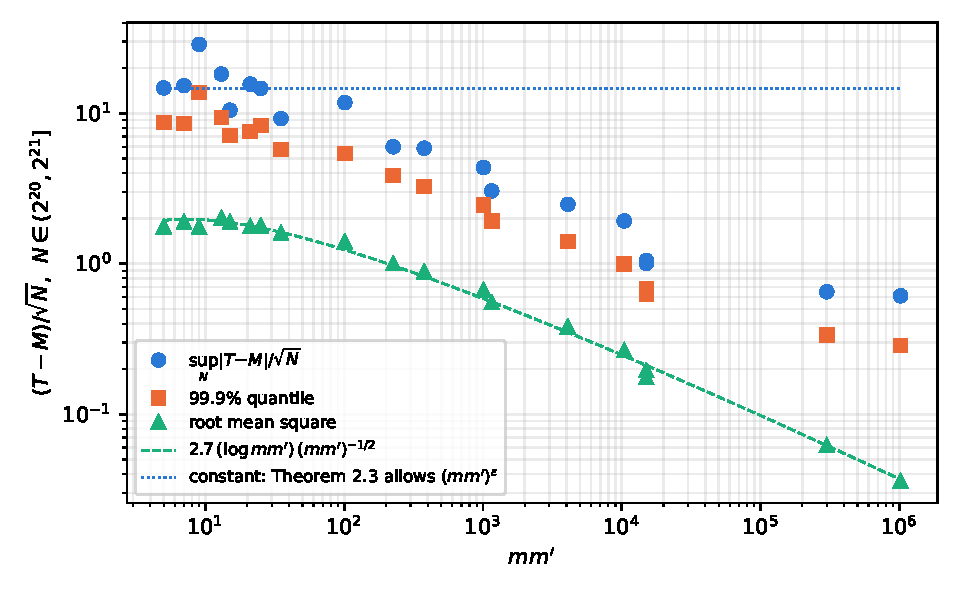
\includegraphics[width=0.66\textwidth]{sup_error.pdf}
\caption{The data of Table~\ref{tab:num} for $X=2^{21}$ (all pairs computed), with the lines $(mm')^{-1/4}$ and $(mm')^{1/4}$ for comparison. The supremum does not grow with the level; the root mean square decreases like $(mm')^{-1/4}$.}
\label{fig:sup}
\end{figure}

\begin{table}[ht]
\centering
\small
\begin{tabular}{rrrrrr}
\hline
$(m,m')$ & $mm'$ & rms & 99.9\% quantile & $\sup$, $X=2^{21}$ & $\sup$, $X=2^{23}$\\
\hline
$(1,5)$ & 5 & 1.76 & 8.7 & 14.7 & 17.3\\
$(9,1)$ & 9 & 1.76 & 13.7 & 28.7 & 33.8\\
$(3,5)$ & 15 & 1.90 & 7.1 & 10.5 & 12.2\\
$(1,101)$ & 101 & 1.40 & 5.4 & 11.8 & 12.1\\
$(13,29)$ & 377 & 0.89 & 3.3 & 5.9 & 6.8\\
$(1,1009)$ & 1009 & 0.67 & 2.5 & 4.4 & 5.3\\
$(61,67)$ & 4087 & 0.38 & 1.4 & 2.5 & 2.4\\
$(101,103)$ & 10403 & 0.27 & 1.0 & 1.9 & 1.8\\
$(1,15015)$ & 15015 & 0.18 & 0.6 & 1.0 & --\\
$(1009,1013)$ & 1022117 & 0.036 & 0.29 & 0.61 & 0.55\\
\hline
\end{tabular}
\medskip
\caption{Statistics of $(T(m,m';N)-M(m,m';N))/\sqrt N$ over all $N\in(X/2,X]$ satisfying \eqref{eq:admissible} ($\approx10^6$ values for $X=2^{21}$, $4\cdot10^6$ for $X=2^{23}$; the run with $X=2^{23}$ covers a selection of the pairs).}
\label{tab:num}
\end{table}

\subsection{Observations}
Two features stand out. First, the root mean square decreases like $(mm')^{-1/4}$. By the Rankin--Selberg method, the mean square of $a_G(n)/\sqrt n$ over $n\le Y$ is asymptotic to an absolute constant times $\|G\|^2/\mathrm{vol}(\Gamma_0(4mm')\backslash\HH)$, and the volume is $\asymp mm'$; so the data say $\|G\|\asymp(mm')^{1/4}$, i.e.\ Lemma~\ref{lem:waibel} appears to be sharp up to $N^\e$. (Waibel's lower bound \cite[Theorem~3]{Waibel} gives only $\|G\|^2\gg1/\min(m,m')$ for our forms.)

Second, the supremum over $N$ does not grow with $mm'$ at all---it decreases---while Theorem~\ref{thm:unif} allows growth like $(mm')^{1/4}$. The gap is the Cauchy--Schwarz step in Lemma~\ref{lem:hecke}. Expanding in an orthogonal basis of Hecke eigenforms (Section~\ref{subsec:auto}), $a_G(N)$ is a sum of $\asymp mm'$ terms $\langle G,f\rangle a_f(N)/\|f\|^2$; Cauchy--Schwarz bounds this sum by $\|G\|$ times the square root of the Petersson sum $\sum_f|a_f(N)|^2/\|f\|^2\asymp N$, and it is attained only if the phases of the individual terms align with those of $\overline{a_f(N)}$. The data are consistent with the opposite: the terms behave like a sum with essentially random signs, whose size is about $(mm')^{-1/4}$ times the Cauchy--Schwarz bound in the root mean square, and does not exceed the size for fixed level in the supremum. The growth in $N$ between $X=2^{21}$ and $2^{23}$ is by a factor $1.0$--$1.2$, as expected from Deligne's bound (the suprema are attained at $N$ with $16$--$96$ divisors).

\subsection{Status of the numerical evidence}
We stress the logical status of these data. They consist of finitely many pairs $(m,m')$ and finitely many $N\le 2^{23}$, and no finite computation can establish a bound that is uniform in $m,m'$ and $N$; in particular the computations do not bear on Theorem~\ref{thm:main}, Theorem~\ref{thm:level} or Theorem~\ref{thm:unif}, which are proved independently of them. The data are compatible with Theorem~\ref{thm:unif} (and with Lemma~\ref{lem:waibel} being sharp), and they are consistent with the factor $(mm')^{1/4}$ being an artefact of the method. They are compatible with, and motivate, the following conjecture; they do not prove it, and they give no information about $N$ or $mm'$ beyond the range computed.

\begin{conjecture}\label{conj}
For coprime odd $m,m'$ and $N\ge1$ with $(N,mm')=1$ and $v_2(N)\le1$,
\[
T(m,m';N)=M(m,m';N)+O_\e\bigl(N^{1/2+\e}\bigr)
\]
uniformly in $m,m'$.
\end{conjecture}

If Conjecture~\ref{conj} holds, then by Lemma~\ref{lem:reduce} the same bound (with an extra factor $4^{\omega(N)}d(N)\le d(N)^3$, which may be absorbed into $N^\e$) holds for cube-free $m,m'$ with $(N,mm')>1$, the proof of Theorem~\ref{thm:level} gives the level of distribution $1/2$ for $r(n)r(N-n)$, and Remark~\ref{rem:half} gives the bounds $8$ and $5$ in place of $9$ and $6$.

\subsection{An automorphic interpretation of Conjecture~\ref{conj}}\label{subsec:auto}
The following discussion is heuristic and is not used anywhere in the paper. Let $L=4mm'$ and let $\mathcal B^*$ be an orthogonal basis of $S_2(\Gamma_0(L))$ consisting of eigenforms of all $T_n$, $(n,L)=1$; by the proof of Lemma~\ref{lem:hecke} it may be taken inside the spaces $S(f)$, so every element $\varphi\in\mathcal B^*$ has $a_\varphi(n)=\lambda_f(n)\,n^{1/2}a_\varphi(1)$ for $(n,L)=1$, where $f$ is the underlying newform and $\lambda_f(n)=a_f(n)n^{-1/2}$. Since $E$ is orthogonal to cusp forms, $\langle\Theta,\varphi\rangle=\langle G,\varphi\rangle$, and for $(N,L)=1$
\begin{equation}\label{eq:spectral}
T(m,m';N)-M(m,m';N)=a_G(N)=\sum_{\varphi\in\mathcal B^*}\frac{\langle\Theta,\varphi\rangle}{\|\varphi\|^2}\,a_\varphi(N)
=N^{1/2}\sum_{\varphi\in\mathcal B^*}\frac{\langle\Theta,\varphi\rangle\,a_\varphi(1)}{\|\varphi\|^2}\,\lambda_f(N).
\end{equation}

\emph{The coefficients $\langle\Theta,\varphi\rangle$.} The form $\theta^2$ is the weight-one Eisenstein series of level $4$ and character $\chi$, with $L$-function $\sum r(n)n^{-s}=4\zeta(s)L(s,\chi)$. Writing $\theta^2(m'z)$ as a combination of weight-one Eisenstein series for the cusps of $\Gamma_0(4m')$ and unfolding (the Rankin--Selberg method in Shimura's form \cite{Shimura}, with Hecke's trick at the holomorphic point), $\langle\theta^2(m\,\cdot)\theta^2(m'\,\cdot),\varphi\rangle$ becomes a combination of values at the centre of Dirichlet series of the shape $\sum_n\overline{\lambda_f(n)}\,r(n)\,n^{-s}$, twisted by the local data at $2mm'$. Since $\sum_n\lambda_f(n)r(n)n^{-s}=4L(s,f)L(s,f\otimes\chi)/\zeta^{(L)}(2s)$ up to Euler factors at the primes dividing $L$, one expects
\begin{equation}\label{eq:RS}
\langle\Theta,\varphi\rangle=\mathcal E_\varphi(m,m')\;L(\tfrac12,f)\,L(\tfrac12,f\otimes\chi),
\end{equation}
with a factor $\mathcal E_\varphi(m,m')$ built from local factors at the primes dividing $2mm'$ and from the normalisation of $\varphi$. We have not worked out $\mathcal E_\varphi$, and \eqref{eq:RS} should be read as a statement about the structure of the coefficients, not as an identity we use. (In particular, it is the product of the two central values that enters linearly, as in the Rankin--Selberg method, not a square root of it as in Waldspurger-type formulas for half-integral weight.)

\emph{Heuristic reformulation.} Assuming the structural factorisation \eqref{eq:RS}, which we have not proved, and inserting it into \eqref{eq:spectral}, the cuspidal error becomes
\begin{gather}
T(m,m';N)-M(m,m';N)=N^{1/2}\,\mathcal S(m,m';N),\notag\\
\mathcal S(m,m';N)=\sum_{\varphi\in\mathcal B^*}\omega_\varphi\,L(\tfrac12,f)\,L(\tfrac12,f\otimes\chi)\,\lambda_f(N),\label{eq:moment}
\end{gather}
with weights $\omega_\varphi=\mathcal E_\varphi(m,m')\,a_\varphi(1)/\|\varphi\|^2$, i.e.\ $N^{1/2}$ times a twisted first moment over a family of $\asymp mm'$ forms of weight $2$ and level $4mm'$. In these terms, Theorem~\ref{thm:unif} is what one gets by bounding $\mathcal S$ through Cauchy--Schwarz, with the second moment of the coefficients $\langle\Theta,\varphi\rangle$ controlled by $\|G\|^2$ (Lemma~\ref{lem:waibel}) and the second moment of $\lambda_f(N)$ controlled by the Petersson formula; this loses all cancellation among the terms of \eqref{eq:moment}, and the loss is $\|G\|\asymp(mm')^{1/4}$. In this heuristic form, Conjecture~\ref{conj} becomes the statement $\mathcal S(m,m';N)\ll_\e N^{\e}$ uniformly, i.e.\ that the sum in \eqref{eq:moment} exhibit cancellation saving $(mm')^{1/4}$ over the Cauchy--Schwarz bound. Since the summands are not of constant sign (because of $\lambda_f(N)$ and of the local factors), this cancellation cannot come from positivity, and a proof along these lines would have to exploit the oscillation of $\lambda_f(N)$ across the family. None of this constitutes a proof of Conjecture~\ref{conj}, or of \eqref{eq:RS}.

\emph{A possible approach.} The standard route to first moments of this kind is to write $L(\frac12,f)L(\frac12,f\otimes\chi)$ by an approximate functional equation of length about the square root of the analytic conductor $\asymp(mm')^2$, i.e.\ about $mm'$, to combine $\lambda_f(a)\lambda_f(N)$ by the Hecke relations, and to average over the family with the Petersson formula (as in the work of Iwaniec and Sarnak \cite{IwaniecSarnak} on first moments with harmonic weights). The diagonal terms are then explicit, and the off-diagonal terms are sums of Kloosterman sums $S(aN,b;c)$ with $c\equiv0\pmod{4mm'}$, to which Weil's bound applies. The main obstacle is that in the range relevant for the level $1/2$ one has $mm'\le N^{1/2}$, so the twist $\lambda_f(N)$ is long compared with the level, and the off-diagonal terms are not small without further cancellation in the sums over $a,b$ and $c$ (for instance from the Kuznetsov formula and bounds for sums of Kloosterman sums). We have not attempted this.

%=====================================================================================================
\appendix
\section{The numerical verification of Lemma~\ref{lem:numerics} and of $c_h$}\label{app:numerics}

This appendix describes precisely what is computed by the two scripts \texttt{certify\_modular.py} and \texttt{singular\_constant.py}. Let $h_0=10^{-3}$ and $s_i=ih_0$. For the closed forms, all interval computations use the interval type \texttt{mpmath.iv} with $80$-bit precision; for the recurrences they use IEEE double precision with one outward \texttt{nextafter} step after every arithmetic operation; we write $\lfloor x\rfloor_\downarrow$ and $\lceil x\rceil^\uparrow$ for the outward-rounded results.

\subsection{The linear sieve functions}\label{app:sieve}
The functions $F_1,f_1$ are determined by
\[
F_1(s)=\frac{2e^\gamma}{s}\ \ (0<s\le3),\qquad f_1(s)=\frac{2e^\gamma\log(s-1)}{s}\ \ (2\le s\le4),
\]
\[
(sF_1(s))'=f_1(s-1)\ \ (s>3),\qquad (sf_1(s))'=F_1(s-1)\ \ (s>2),
\]
and $F_1$ is decreasing, $f_1$ increasing on their domains \cite[Chapter~11]{FI}. On the grid points $s_i\le3$ (resp.\ $2<s_i\le4$) enclosures $[F^-_i,F^+_i]$ (resp.\ $[f^-_i,f^+_i]$) are obtained by evaluating the closed forms in interval arithmetic. For larger $s$ we integrate the delay equations over one grid cell. With $G_F(s)=sF_1(s)$, $G_f(s)=sf_1(s)$ and $j=i-1000$ (so $s_j=s_i-1$),
\[
G_F(s_{i+1})-G_F(s_i)=\int_{s_i}^{s_{i+1}}f_1(s-1)\,\dd s\in\bigl[h_0\,f_1(s_j),\ h_0\,f_1(s_{j+1})\bigr],
\]
because $f_1$ is increasing, and
\[
G_f(s_{i+1})-G_f(s_i)=\int_{s_i}^{s_{i+1}}F_1(s-1)\,\dd s\in\bigl[h_0\,F_1(s_{j+1}),\ h_0\,F_1(s_j)\bigr],
\]
because $F_1$ is decreasing. Replacing the values on the right by their enclosures gives the one-step recursion
\begin{align*}
G^-_F(s_{i+1})&=\lfloor G^-_F(s_i)+h_0^-f^-_j\rfloor_\downarrow, & G^+_F(s_{i+1})&=\lceil G^+_F(s_i)+h_0^+f^+_{j+1}\rceil^\uparrow,\\
G^-_f(s_{i+1})&=\lfloor G^-_f(s_i)+h_0^-F^-_{j+1}\rfloor_\downarrow, & G^+_f(s_{i+1})&=\lceil G^+_f(s_i)+h_0^+F^+_{j}\rceil^\uparrow,
\end{align*}
starting from the interval values at $s=3$ and $s=4$, and
\[
F^-_{i+1}=\bigl\lfloor G_F^-(s_{i+1})/s_{i+1}^+\bigr\rfloor_\downarrow,\qquad F^+_{i+1}=\bigl\lceil G_F^+(s_{i+1})/s_{i+1}^-\bigr\rceil^\uparrow,
\]
and similarly for $f^\pm_{i+1}$. Here $[s_i^-,s_i^+]$ is the enclosure of $s_i=i/1000$, and $h_0^-=\lfloor s_{i+1}^--s_i^+\rfloor_\downarrow$, $h_0^+=\lceil s_{i+1}^+-s_i^-\rceil^\uparrow$ are the lower and upper enclosures of the step $s_{i+1}-s_i$; the lower enclosure is used in the formulas for $G^-$ and the upper one in those for $G^+$ (all factors $f^\pm_j$, $F^\pm_j$ being non-negative). This is a one-step enclosure, not an iteration to a fixed point: since the delay is exactly $1000$ grid steps, the values needed on the right have always been computed earlier. By induction $F_1(s_i)\in[F^-_i,F^+_i]$ and $f_1(s_i)\in[f^-_i,f^+_i]$ for $s_i\le60$. The enclosures are narrow: the computation gives $F_1(3),f_1(4)$ to six decimals, and $F_1(60)\le1.000066$, $f_1(60)\ge0.999935$, in agreement with $F_1,f_1\to1$.

Off the grid, monotonicity gives
\[
F_1(s)\le F^+_{\lfloor s/h_0\rfloor-1},\qquad F_1(s)\ge F^-_{\lceil s/h_0\rceil+1},\qquad f_1(s)\ge f^-_{\lfloor s/h_0\rfloor-1}
\]
(the extra index shift guards against the rounding of $s/h_0$), and $F_1(s)\le\lceil 2e^\gamma/s\rceil^\uparrow$ for $s\le3$.

\subsection{The bounds for $L$ and $R$}\label{app:LR}
\emph{The lower bound for $L$.} We write $L=f_1(s_A)F_1(s_B)+F_1(s_A)\bigl(f_1(s_B)-F_1(s_B)\bigr)$. Since $f_1(s_B)-F_1(s_B)\le0$, a lower bound is
\[
L\ge f_1^-(s_A)\,F_1^-(s_B)+F_1^+(s_A)\,\bigl(f_1^-(s_B)-F_1^+(s_B)\bigr),
\]
with the off-grid bounds of Section~\ref{app:sieve} and outward rounding. The split $\theta_A$ is a free parameter; the script scans $801$ values in $[0.3\theta,0.7\theta]$ in floating point, keeps the best, and then evaluates the lower bound rigorously at that value. This gives $L\ge0.998974$ for $\alpha=9/250$ ($\theta_A=0.1998$, $s_A=5.5500$, $s_B=5.5611$).

\emph{The upper bound for $R$.} Divide $[\alpha,\beta_1]$ into $K=4000$ cells $[u_k,u_{k+1}]$, $u_k=\alpha+k(\beta_1-\alpha)/K$ (enclosed outward). On a cell:
\begin{itemize}[leftmargin=2em]
\item the factor $(1-u/\beta_1)/u$ is decreasing in $u$, hence at most its value at $u_k$;
\item $U(t)$ is non-increasing in $t$, because $F_1$ is decreasing; so $U(\theta-u)\le U(\theta-u_{k+1})$ on the cell;
\item $U(t)\le F_1(t'/\alpha)F_1((t-t')/\alpha)$ for every admissible $t'$, since $U$ is a minimum; the script takes the smallest of these upper bounds over $81$ values $t'\in[0.3t,0.7t]$, each evaluated with $F_1^+$.
\end{itemize}
Hence
\[
R\le 2\sum_{k=0}^{K-1}\Bigl\lceil\frac{1-u_k/\beta_1}{u_k}\Bigr\rceil^\uparrow\cdot\min_{t'}F^+_1\Bigl(\frac{t'}{\alpha}\Bigr)F^+_1\Bigl(\frac{\theta-u_{k+1}-t'}{\alpha}\Bigr)\cdot(u_{k+1}-u_k),
\]
every operation rounded upwards. For the first line of Table~\ref{tab:cert} this gives $R\le2.816690$, and then $L-\lambda R\ge0.153967$ with $\lambda$ rounded upwards. The other lines of Table~\ref{tab:cert} and the conditional values of Remark~\ref{rem:half} are obtained in the same way.

The verification certifies the numerical inequality $L-\lambda R>0$ only. The sieve lemmas behind Proposition~\ref{prop:W} and the $o(1)$ terms are proved, not computed.

\subsection{The constant $c_h$}\label{app:ch}
Let $P_1(z)=\prod_{p<z,\ p\equiv1\,(4)}(1-1/p)$. Mertens' theorem $\prod_{p<z}(1-1/p)\sim e^{-\gamma}/\log z$ and the convergence of $\prod_p(1-\chi(p)/p)$ to $L(1,\chi)^{-1}=4/\pi$ give
\[
P_1(z)^2=\frac{\prod_{p<z}(1-1/p)\,\prod_{p<z}(1-\chi(p)/p)}{(1-\frac12)\prod_{q<z}(1-q^{-2})}\sim\frac{2e^{-\gamma}}{\kappa\log z},\qquad
\kappa=\frac\pi4\prod_{q\equiv3\,(4)}\Bigl(1-\frac1{q^2}\Bigr).
\]
Writing $\prod_{2<p<z}(1-h(p))=P_1(z)^2\,C(z)$ with
\[
C(z)=\prod_{\substack{p<z\\ p\equiv1\,(4)}}\Bigl(1+\frac{2p-1}{(p+1)(p-1)^2}\Bigr)\prod_{\substack{q<z\\ q\equiv3\,(4)}}\Bigl(1-\frac1{q(q-1)}\Bigr)
\]
(for split $p$, $(1-h(p))(1-1/p)^{-2}=p(p^2-p+1)/((p+1)(p-1)^2)$), we get the exact identity $c_h=(2e^{-\gamma}/\kappa)\,C(\infty)$; both infinite products converge absolutely, their factors being $1+O(p^{-2})$.

We compute the products over the primes $p\le P=10^7$ in double precision by summing logarithms, and bound the tails as follows. For $p>P$ the logarithms of the factors are at most $2.01/p^2$ in absolute value (for the split factors, $(2p-1)/((p+1)(p-1)^2)<2.01/p^2$ for $p>10^7$, and for the others $|\log(1-x)|\le x(1+x)$ with $x\le1.01/p^2$), and
\[
\sum_{p>P}\frac1{p^2}<\sum_{n>P}\frac1{n^2}<\frac1P .
\]
Hence the tails of $\log\kappa$ and of $\log C(\infty)$ lie in $[-1.01/P,0]$ (its factors are $1-q^{-2}$) and $[-2.01/P,2.01/P]$ respectively; the script uses the wider margins $2/P$ for $\log\kappa$ and $4/P$ for $\log C(\infty)$. The rounding error of the double-precision summation over the $\approx6.6\cdot10^5$ primes is of relative size $10^{-10}$, far inside these margins. This gives
\[
\kappa\in[0.67238629,\,0.67238642],\qquad C(\infty)\in[0.89899105,\,0.89899177],
\]
and hence $c_h\in[1.501360,\,1.501362]$.
This computation is in floating point with explicit margins rather than in interval arithmetic; since $c_h$ enters only the value of the constant $c_1$ in Theorem~\ref{thm:main}, and not the positivity of $L-\lambda R$, this suffices. As a rough independent check, $(\log P)\prod_{2<p<P}(1-h(p))=1.50132$, consistent with $c_h$ and with the $O(1/\log P)$ rate of convergence.

%=====================================================================================================
\section*{Data and code availability}
{\sloppy
The scripts behind Table~\ref{tab:num} and Figure~\ref{fig:sup} (\texttt{sup\_error\_scan.py}), Table~\ref{tab:cert} (\texttt{certify\_modular.py}), the choice of the sieve parameters (\texttt{modular\_sieve\_scan.py}) and the constant $c_h$ (\texttt{singular\_constant.py}), together with their outputs, are available at
\begin{center}
\url{https://github.com/Ruqing1963/two-squares-theta-level}
\end{center}
and archived at Zenodo, \href{https://doi.org/10.5281/zenodo.23438288}{doi:10.5281/zenodo.23438288}. The numbers in the paper are those printed in the output files of the repository: Table~\ref{tab:cert} and Remark~\ref{rem:half} in \texttt{results/certify\_modular\_output.txt} and \texttt{results/certify\_modular\_output\_half.txt}; Table~\ref{tab:num} and Figure~\ref{fig:sup} in \texttt{results/sup\_error\_scan\_x21.txt} and \texttt{results/sup\_error\_scan\_x23.txt}; the constant $c_h$ and $c_1$ in \texttt{results/singular\_constant\_output.txt}. The certification of Lemma~\ref{lem:numerics} uses directed rounding; the experiments of Section~\ref{sec:numerics} use floating point and are not certified.
\par}

\indent During the preparation of this work the author used the Claude language model and the \texttt{mpmath} Python library for the computer-assisted interval arithmetic verification of Section~\ref{sec:sieve} and for the numerical experiments of Section~\ref{sec:numerics}. All analytical derivations and proofs were independently audited and verified by the author.

\begin{thebibliography}{99}
\bibitem{AL} A.~O.~L.~Atkin, J.~Lehner, \emph{Hecke operators on $\Gamma_0(m)$}, Math. Ann. \textbf{185} (1970), 134--160.
\bibitem{BF} J.~Br\"udern, \'E.~Fouvry, \emph{Lagrange's four squares theorem with almost prime variables}, J. reine angew. Math. \textbf{454} (1994), 59--96.
\bibitem{Chen2} R.~Chen, \emph{Even integers as sums of two sums of two squares with few prime factors}, preprint (2026), \href{https://doi.org/10.5281/zenodo.23137626}{doi:10.5281/zenodo.23137626}.
\bibitem{Deligne} P.~Deligne, \emph{La conjecture de Weil. I}, Inst. Hautes \'Etudes Sci. Publ. Math. \textbf{43} (1974), 273--307.
\bibitem{FI} J.~Friedlander, H.~Iwaniec, \emph{Opera de Cribro}, Amer. Math. Soc. Colloq. Publ. \textbf{57}, 2010.
\bibitem{IK} H.~Iwaniec, E.~Kowalski, \emph{Analytic Number Theory}, Amer. Math. Soc. Colloq. Publ. \textbf{53}, 2004.
\bibitem{ILS} H.~Iwaniec, W.~Luo, P.~Sarnak, \emph{Low lying zeros of families of $L$-functions}, Inst. Hautes \'Etudes Sci. Publ. Math. \textbf{91} (2000), 55--131.
\bibitem{IwaniecRosser} H.~Iwaniec, \emph{Rosser's sieve}, Acta Arith. \textbf{36} (1980), 171--202.
\bibitem{IwaniecSarnak} H.~Iwaniec, P.~Sarnak, \emph{The non-vanishing of central values of automorphic $L$-functions and Landau--Siegel zeros}, Israel J. Math. \textbf{120} (2000), 155--177.
\bibitem{IwaTopics} H.~Iwaniec, \emph{Topics in Classical Automorphic Forms}, Grad. Stud. Math. \textbf{17}, Amer. Math. Soc., 1997.
\bibitem{KimSarnak} H.~H.~Kim, \emph{Functoriality for the exterior square of $\mathrm{GL}_4$ and the symmetric fourth of $\mathrm{GL}_2$}, with appendix~1 by D.~Ramakrishnan and appendix~2 by H.~H.~Kim and P.~Sarnak, J. Amer. Math. Soc. \textbf{16} (2003), 139--183.
\bibitem{Kitaoka} Y.~Kitaoka, \emph{A note on Hecke operators and theta-series}, Nagoya Math. J. \textbf{42} (1971), 189--195.
\bibitem{Shimura} G.~Shimura, \emph{The special values of the zeta functions associated with cusp forms}, Comm. Pure Appl. Math. \textbf{29} (1976), 783--804.
\bibitem{Siegel} C.~L.~Siegel, \emph{\"Uber die analytische Theorie der quadratischen Formen}, Ann. of Math. (2) \textbf{36} (1935), 527--606.
\bibitem{Top} B.~Topacogullari, \emph{On a certain additive divisor problem}, Acta Arith. \textbf{181} (2017), 143--172; \href{https://arxiv.org/abs/1512.05770}{arXiv:1512.05770}.
\bibitem{Waibel} F.~Waibel, \emph{Uniform bounds for norms of theta series and arithmetic applications}, Math. Proc. Cambridge Philos. Soc. \textbf{173} (2022), 669--691.
\end{thebibliography}

\end{document}
